\documentclass[a4paper,10pt]{article}

% === Encoding & Sprache ===
\usepackage[T1]{fontenc}
\usepackage[utf8]{inputenc}
\usepackage[english]{babel}
\usepackage{newunicodechar}
\usepackage{comment}
\newunicodechar{−}{-}


% === Schrift ===
\usepackage{helvet} % Helvetica verfügbar
\renewcommand{\familydefault}{\sfdefault} % sans-serif font type (in printed versions serif is easier to read, in digital form sans-serif is easier to read)

% === Mathematik & Chemie ===
\usepackage{amsmath,amssymb,bm}
\usepackage{chemformula}

% === Seitenlayout ===
\usepackage[left=2cm,right=2cm,top=2.8cm,bottom=2.8cm]{geometry}
\usepackage{rotating}

% === Tabellen & Spalten ===
\usepackage{array}
\usepackage{tabularx}
\usepackage{caption} % put in preamble
\usepackage{capt-of}
\usepackage{booktabs}
\usepackage{longtable}
\usepackage{multirow}
\usepackage{threeparttable}
\newcolumntype{Y}{>{\centering\arraybackslash}X}
% Flexible Spalten (einheitliche L-Definition)
\newcolumntype{L}[1]{>{\RaggedRight\arraybackslash\hspace{0pt}}p{\dimexpr#1-2\tabcolsep\relax}}

% === Grafiken & Abbildungen ===
\usepackage{graphicx}
\usepackage{adjustbox}
\usepackage{wrapfig}
\usepackage{sidecap}
\usepackage{svg}
\usepackage{tikz}
\usepackage{subcaption}
\usepackage{pdflscape}
\usepackage{url}
\usepackage{pdfpages}

% === Farben (cleaned version) ===
\usepackage[table,dvipsnames,svgnames]{xcolor} % core color package
\usepackage{xkcdcolors}                        % optional xkcd color palette

% --- Custom ESA / project colors ---
\definecolor{ESAblue}{RGB}{0,56,168}
\definecolor{ESAgreen}{RGB}{0,150,0}
\definecolor{ESAred}{RGB}{200,0,0}
\definecolor{hummocky}{RGB}{79,189,255}
\definecolor{mottled}{RGB}{255,179,0}
\definecolor{angular}{RGB}{157,60,255}
\definecolor{powder}{RGB}{255,68,171}
\definecolor{Bennu}{RGB}{0,0,255}
\definecolor{Poster}{RGB}{55,55,255}
\definecolor{Perseuss}{RGB}{46,139,87}
\definecolor{perseuss}{RGB}{80,200,120}
\definecolor{headbg}{HTML}{F0F3F7}
\definecolor{bandbg}{HTML}{FAFAFA}
\definecolor{Laser}{RGB}{136,193,74}
\definecolor{LASERfinal}{RGB}{82,186,158}

% --- Optional standard colors to avoid undefined errors ---
% These define safe, capitalized versions in case any package or comment uses them
\definecolor{RED}{named}{red}
\definecolor{GREEN}{named}{green}
\definecolor{BLUE}{named}{blue}
\definecolor{BLACK}{named}{black}

% --- Cell header command for tables ---
\newcommand{\thdr}[1]{\cellcolor{headbg}\textbf{#1}}


% === Beschriftungen ===
\usepackage{caption}
\captionsetup{font=small}
\captionsetup[figure]{labelfont={bf},name={Fig.},labelsep=period}
\captionsetup[table]{labelfont={bf},name={Table},labelsep=period}
\captionsetup[subfigure]{width=0.9\textwidth}

% === Einheiten & Symbole ===
\usepackage{siunitx}
\DeclareSIUnit\year{a}
\usepackage{gensymb}
\usepackage{wasysym}
\usepackage{textcomp}

% === Verweise & Literatur ===
% === Verweise & Literatur ===
\usepackage[numbers,square]{natbib}
\usepackage[nottoc]{tocbibind}
\usepackage[colorlinks,bookmarks=false,linkcolor=purple,
            urlcolor=blue,citecolor=purple]{hyperref}
\usepackage{cleveref}
\crefname{table}{Table}{Tables}
\crefname{section}{Section}{Sections}
\crefname{figure}{Fig.}{Figs.}
\crefname{equation}{Eq.}{Eqs.}
\Crefname{figure}{Figure}{Figures}




% === Anhänge ===
\usepackage[titletoc]{appendix}

% === Listen, Floats, Satz ===
\usepackage{enumitem}
\usepackage{float}
\usepackage{ragged2e}
\usepackage{parskip}
\setlength{\parindent}{1cm}
\usepackage{setspace}
\setstretch{1.25}
\usepackage[normalem]{ulem}
\usepackage{lipsum}

% === Abschnittstitel & Boxen ===
\usepackage[explicit]{titlesec}
\usepackage{tcolorbox}
% --- Define box styles ---
\tcbset{
  bluetitle/.style={
    enhanced,
    colback=perseuss,
    colframe=white,
    boxrule=0.5pt,
    width=\textwidth,
    left=6pt, right=6pt, top=4pt, bottom=0pt,
    arc=2pt,
    boxsep=0pt,
    enlarge bottom by=-10pt
  },
  chaptertitle/.style={
    enhanced,
    colback=Perseuss,
    colframe=white,
    boxrule=0.5pt,
    width=\textwidth,
    left=6pt, right=6pt, top=4pt, bottom=0pt,
    arc=2pt,
    boxsep=0pt,
    enlarge bottom by=-10pt
  },
  whitesubtitle/.style={
    enhanced,
    colback=white,
    colframe=blue!50!black,
    boxrule=0.5pt,
    width=\textwidth,
    left=6pt, right=6pt, top=3pt, bottom=3pt,
    arc=0pt,
    boxsep=0pt,
    enlarge top by=-0.5pt
  }
}

% === Kopf- und Fußzeilen ===
\usepackage{fancyhdr}
\pagestyle{fancy}
\fancyhead{}
\fancyfoot[LO,RE]{}
\fancyfoot[LE,RO]{}
\fancyhead[LE,RO]{FS26%\leftmark}
}
\fancyhead[C]{}
\fancyhead[LO,RE]{Space Data Project 3}
\fancyfoot[C]{\thepage}

% === Zähler & Tiefen ===
\setcounter{secnumdepth}{4}
\setcounter{tocdepth}{4}

% === Absatzformatierung ===
\makeatletter
\renewcommand\paragraph{\@startsection{paragraph}{4}{\z@}%
  {3ex plus .2ex minus 0ex}{1ex}%
  {\normalfont\normalsize\bfseries}}
\makeatother

% === Doppelseitenumbruch anpassen ===
\makeatletter
\def\cleardoublepage{\clearpage\if@twoside \ifodd\c@page\else
\hbox{}
\vspace*{\fill}
\thispagestyle{empty}
\newpage
\if@twocolumn\hbox{}\newpage\fi\fi\fi}
\makeatother

% === Tabellenabstände ===
\renewcommand{\arraystretch}{1.02}
\setlength{\tabcolsep}{4pt}
\setlength{\extrarowheight}{0pt}

% === Sonstige Makros ===
\newcommand{\tbd}{\textbf{TBD}}
\newcommand{\otoprule}{\midrule[\heavyrulewidth]}
\newcommand*\rot{\rotatebox{90}}
\newcommand{\fathline}{\rule{\linewidth}{0.5mm}}
\newcommand\nobrkhyph{\mbox{-}}
\widowpenalty=9999
\clubpenalty=9999

% Farbige S-Zellen (gelassen wie vorgegeben)
\renewcommand{\S}[1]{%
  \begingroup
  \def\n{#1}%
  \ifcase\n\relax
    \cellcolor{white}\textbf{#1}%
  \or
    \cellcolor{red!70}\textbf{1}%
  \or
    \cellcolor{red!40!yellow}\textbf{2}%
  \or
    \cellcolor{yellow!65}\textbf{3}%
  \or
    \cellcolor{green!35!yellow}\textbf{4}%
  \or
    \cellcolor{green!65}\textbf{5}%
  \else
    \cellcolor{white}\textbf{#1}%
  \fi
  \endgroup
}

% ------- alternative title formatting (als Kommentar belassen) ------
\begin{comment}
\titleformat{\chapter}[display]
  {\Huge\scshape}
  {\filleft\tikz\node[fill=green!50!black!10,rectangle,rounded corners=6pt] (chap) {\chaptertitlename};}
  {0ex}
  {\colorbox{green!50!black!10}{\parbox{\dimexpr\textwidth-2\fboxsep\relax}{\vskip1ex#1\vskip1ex}}}
\end{comment}

\begin{comment}
% define some colors
\definecolor{section}{RGB}{10,221,164}
\definecolor{subsection}{RGB}{200,255,240}
\definecolor{titletext}{RGB}{0,0,0}
\definecolor{turkis}{RGB}{2,159,106}

% section color box
\setkomafont{section}{\mysection}
\newcommand{\mysection}[1]{%
	\Large\sf%
	\setlength{\fboxsep}{0cm}%
	\colorbox{section}{%
		\begin{minipage}{\linewidth}%
			\vspace*{2pt}%
			\leftskip2pt
			\rightskip\leftskip
			{\color{titletext} #1}
			\vspace*{1pt}%
		\end{minipage}%
}}

% subsection color box
\setkomafont{subsection}{\mysubsection}
\newcommand{\mysubsection}[1]{%
	\Large\sf%
	\setlength{\fboxsep}{0cm}%
	\colorbox{subsection}{%
		\begin{minipage}{\linewidth}%
			\vspace*{2pt}%
			\leftskip2pt
			\rightskip\leftskip
			{\color{titletext} #1}
			\vspace*{1pt}%
		\end{minipage}%
}}
\end{comment}

% ------------ alternative (als Kommentar belassen) ---------
\begin{comment}
\titleformat{\section}
  {\Large\rmfamily\bfseries\color{Perseuss}}{\thesection}{1em}{#1}

\titleformat{\subsection}
  {\Large\rmfamily\bfseries\color{perseuss}}{\thesection}{1em}{#1}
\end{comment}

% ------- Hinweise / alte, auskommentierte Zeilen beibehalten -------
% \usepackage[comma]{natbib}
% \usepackage{graphicx}


\begin{document}


% ====== Indentation (no stupid indentation :) ) 
\setlength{\parindent}{0pt}

% TITLE PAGE ########################
\begin{comment}
\newgeometry{top=1.5cm, bottom=1.5cm, left=2cm, right=2cm}
\begin{titlepage}
\pagenumbering{gobble} 
\thispagestyle{empty}
\noindent 
\includegraphics[scale=0.2]{Figures/Figures General/eth logo.png} 
%\hfill\includegraphics[scale=0.68]{}
\begin{singlespace}  
%\vspace{-10pt} 
\noindent 
\begin{center} 
    \includegraphics[height=13cm]{Figures/la plata basin.jpg} 
\end{center} 
%\begin{center}
%    \textbf{\LARGE{\textcolor{perseuss}{PERSEUSS\\ 
%    \rule{\linewidth}{.2pt} 
%    \large 
%    \textcolor{perseuss}{Photon-based Explorational Reconnaissance of Sublunar Environments, Underground Structures and Surfaces\\ Mission Project Analysis}}}}
%\end{center}

\begin{center}
    \textbf{ 
    \rule{\linewidth}{.4pt}\\
    \vspace{8pt}
    \large 
    \textcolor{purple}{El Niño vs La Niña Effects in the La Plata Basin}\\
    \vspace{3pt} 
    \rule{\linewidth}{.4pt}\\
    \vspace{5pt}
    \textcolor{purple}{How do El Niño and La Niña differently affect terrestrial water storage in the La Plata Basin in terms of spatial pattern and magnitude? }}
\end{center}
\vspace{25pt} 
\noindent 
\begin{minipage}[t]{0.45\textwidth} 
    \textbf{Authors:}\\ 
    Stasha Petrovikj\\
    Isabel Reinecke\\  
\end{minipage} 
\hfill 
\begin{comment}
\begin{minipage}[t]{0.45\textwidth} 
    \raggedleft 
    \textbf{Supervisors:}\\ 
    Prof. Thomas Zurbuchen\\
    Dr. Simon Stähler\\ 
    Dr. Florian Kehl\\   
\end{minipage}

\vspace{18pt} 
\noindent 
\vspace{0.5cm}
\textbf{\today}
\end{singlespace}
\vspace{40pt} 
\includegraphics[scale=0.25]{Figures/Figures General/eth space logo 2 2.png}\hfill{\includegraphics[scale=0.125]{Figures/Figures General/eaps logo.png}}

\begin{flushleft} 
    \includegraphics[scale=0.22]{Figures/Figures General/eth space logo 2 2.png} 
\end{flushleft} 
\vspace{-30pt}\centering\includegraphics[scale=0.13]{Figures/Figures General/eaps logo.png} 

\hfill\vspace{20pt}\includegraphics[scale=0.18]{Figures/Figures General/logo orb vel 2.png}


\end{titlepage}
\restoregeometry
\end{comment}
%######### MISSION SUMMARY TABLE ################



%######## AUTHORSHIP AND ACKNOWLEDGEMENTS #################

\newpage
\setstretch{1}
\begin{comment}
    

\section*{Authorship and Acknowledgments}
\thispagestyle{plain}
\subsubsection*{Team}
    Author A\\
    Author B\\
    Author C\\  

\subsection*{Acknowledgements}

\textcolor{red}{We would like to thank...}

\end{comment}
\vspace{-30pt}
\begin{center}
    \textbf{ 
    %\rule{\linewidth}{.4pt}\\
    %\vspace{8pt}
    \huge 
    \textcolor{purple}{Denoising PSRs with CNNs}\\
    %\vspace{3pt} 
    \rule{\linewidth}{.4pt}\\
    \vspace{5pt}
    \textcolor{purple}{\normalsize{Mattia De Martino - Isabel Reinecke - Marius Riesterer }}}
\end{center}


% LIST OF CONTENTS, FIGURES AND TABLES ########################

\begin{comment}
    

{\hypersetup{linkcolor=black}
\setcounter{tocdepth}{3}
\tableofcontents}


{\hypersetup{linkcolor=black}
\listoffigures}
%\newpage
%\newpage
%{\hypersetup{linkcolor=black}
%\listoftables}


 % You may want to start the first section on a new page


\end{comment}
% CHAPTERS ########################
% \input{List of Acronyms}
 
% start page numbering at page 1
\pagenumbering{arabic}\setcounter{page}{1}
\section{Introduction}
Denoising of lunar images is essential for improving the reliability of scientific analysis by reducing sensor, transmission, and environmental noise inherent in space imaging. Noise can obscure or distort fine-scale surface features such as small craters and regolith textures, leading to inaccuracies in morphological interpretation. Effective denoising enhances the precision of quantitative measurements, including crater counting and topographic assessments. It also improves the performance of automated image-processing algorithms used in tasks such as feature detection and landing site evaluation.
Starting from a baseline model, we investigate improvements in network architecture, optimization methods, and loss functions in order to denoise high-resolution, noisy images, using the most effective machine learning approach. Different configurations are explored to assess how design choices and hyperparameters influence performance. The models are trained on GPU systems to ensure computational efficiency and scalability. Performance is evaluated using cross-validation and comparisons of training and test losses. Qualitative results are further examined through visualizations of clean, noisy, and denoised images. Overall, the objective is to identify reliable strategies for image denoising and to better understand the associated challenges.

%\section{Objectives}
\section{Method}
In order to find a suitable model for the denoising task, three overall architecture 
categories were chosen based on literature research \cite{10.1007/978-3-319-24574-4_28}, 
\cite{Oktayetal2018}, \cite{TIAN2020251}. We used these references as motivation for 
a standard U-Net family, an attention-gated U-Net family, and residual CNN denoisers. 
In addition, we tested deeper U-Net variants, autoencoders, DINOv2-based feature 
decoders, and conditional diffusion models as higher-risk alternatives.
Each of these models feature distinct architectural differences. The U-Net uses a 
classic encoder-decoder structure with skip connections between the corresponding 
layers. The Attention U-Net extends this by incorporating attention gates to suppress 
irrelevant features in skip connections. Finally, the ResNet model operates at full 
resolution using stacked residual blocks, relying on deep feature extraction rather 
than multi-scale encoding.
Based on these approaches to solve the image denoising problem, we implemented our 
own baseline versions of these models, which architectures are explained in detail in 
Section \ref{sec:model_arch}.\\
Given the number of tunable hyperparameters, we first started with ablation studies, 
as it would be computationally inefficient to test all different combinations. 
Therefore, we used the baseline implementations to vary one parameter at a time to 
get an idea of the optimal model setup for this problem. Throughout the ablation 
studies, we varied the network capacity, the depth of the network architecture, the 
loss function, the optimizer, and the output function. After finishing the ablations, 
we combined the most promising combinations and selected the best performing models 
to perform Bayesian hyperparameter optimization with Optuna \cite{7352306}, to further fit the models to our 
specific problem. Optuna samples hyperparameters from a defined search space, trains 
one trial for a limited budget, evaluates validation PSNR, and uses a median pruner 
to stop trials whose intermediate validation score is clearly below the study median. 
For the Deep U-Net search, we varied feature scale, dropout, output activation, 
learning rate, weight decay, optimizer, and batch size.\\
In parallel, we also developed custom approaches to compare against the standard image 
denoising approaches. The first consists of a DINOv2 \cite{oquab:hal-04376640} feature 
extractor (ViT-L backbone) that divides the image into patches, which are encoded into 
feature vectors. These were then fed into an image decoder head, which was trained on 
our dataset. The second custom approach was inspired by the diffusion approach proposed 
by Ho et al. \cite{ho2020ddpm} for generative image networks. This model is trained by 
adding increasing amounts of noise to an input image, with the model's objective being 
to predict the noise added to the image. This approach seems inherently suited to our 
specific scenario and we therefore compared it to the other networks.




% In order to achieve the most effective denoising, three different machine learning architectures were implemented and evaluated, allowing for a comprehensive and comparative analysis. These three architectures were evaluated: a baseline U-Net, an Attention U-Net, and a ResNet-based denoiser. The U-Net follows a symmetric encoder–decoder structure with skip connections, enabling the preservation of spatial information. The Attention U-Net extends this by incorporating attention gates to suppress irrelevant features in skip connections. Finally, the ResNet model operates at full resolution using stacked residual blocks, relying on deep feature extraction rather than multi-scale encoding.
\subsection{Model Architectures}
\label{sec:model_arch}
% Required packages:
% \usepackage{booktabs}
% \usepackage{multirow}

\begin{table}[H]
\centering
\caption{U-Net Model Architecture Specifications}
\begin{tabular}{lllr}
\toprule
\textbf{Stage} & \textbf{Layer Name} & \textbf{Operation / Output Shape} & \textbf{Parameters} \\
\midrule
\multirow{4}{*}{Encoder}
& input & Grayscale input $(1,64,64)$ & 0 \\
& enc1 & DoubleConv $(64,64,64)$ & 37,696 \\
& enc2 & MaxPool + DoubleConv $(128,32,32)$ & 221,696 \\
& enc3 & MaxPool + DoubleConv $(256,16,16)$ & 885,760 \\
\midrule
Bottleneck
& bottleneck & MaxPool + DoubleConv $(512,8,8)$ & 3,540,992 \\
\midrule
\multirow{6}{*}{Decoder}
& up3 & ConvTranspose2D $(256,16,16)$ & 524,544 \\
& dec3 & Concatenate skip + DoubleConv $(256,16,16)$ & 1,770,496 \\
& up2 & ConvTranspose2D $(128,32,32)$ & 131,200 \\
& dec2 & Concatenate skip + DoubleConv $(128,32,32)$ & 442,880 \\
& up1 & ConvTranspose2D $(64,64,64)$ & 32,832 \\
& dec1 & Concatenate skip + DoubleConv $(64,64,64)$ & 110,848 \\
\midrule
Output
& out\_conv & $1\times1$ Conv2D + Sigmoid $(1,64,64)$ & 65 \\
\midrule
\multicolumn{3}{r}{\textbf{Total Trainable Parameters}} & \textbf{7,699,009} \\
\bottomrule
\end{tabular}
\end{table}


\begin{table}[H]
\centering
\caption{Attention U-Net Model Architecture Specifications}
\begin{tabular}{lllr}
\toprule
\textbf{Stage} & \textbf{Layer Name} & \textbf{Operation / Output Shape} & \textbf{Parameters} \\
\midrule
\multirow{4}{*}{Encoder}
& input & Grayscale input $(1,64,64)$ & 0 \\
& enc1 & DoubleConv $(64,64,64)$ & 37,696 \\
& enc2 & MaxPool + DoubleConv $(128,32,32)$ & 221,696 \\
& enc3 & MaxPool + DoubleConv $(256,16,16)$ & 885,760 \\
\midrule
Bottleneck
& bottleneck & MaxPool + DoubleConv $(512,8,8)$ & 3,540,992 \\
\midrule
\multirow{9}{*}{Decoder}
& up3 & ConvTranspose2D $(256,16,16)$ & 524,544 \\
& att3 & Attention gate on encoder skip $(256,16,16)$ & 66,435 \\
& dec3 & Concatenate attended skip + DoubleConv $(256,16,16)$ & 1,770,496 \\
& up2 & ConvTranspose2D $(128,32,32)$ & 131,200 \\
& att2 & Attention gate on encoder skip $(128,32,32)$ & 16,835 \\
& dec2 & Concatenate attended skip + DoubleConv $(128,32,32)$ & 442,880 \\
& up1 & ConvTranspose2D $(64,64,64)$ & 32,832 \\
& att1 & Attention gate on encoder skip $(64,64,64)$ & 4,323 \\
& dec1 & Concatenate attended skip + DoubleConv $(64,64,64)$ & 110,848 \\
\midrule
Output
& out\_conv & $1\times1$ Conv2D + Sigmoid $(1,64,64)$ & 65 \\
\midrule
\multicolumn{3}{r}{\textbf{Total Trainable Parameters}} & \textbf{7,786,602} \\
\bottomrule
\end{tabular}
\end{table}


\begin{table}[H]
\centering
\caption{ResNet Denoiser Model Architecture Specifications}
\begin{tabular}{lllr}
\toprule
\textbf{Stage} & \textbf{Layer Name} & \textbf{Operation / Output Shape} & \textbf{Parameters} \\
\midrule
Input
& input & Grayscale input $(1,64,64)$ & 0 \\
\midrule
Feature Extraction
& head & Conv2D + BatchNorm + ReLU $(64,64,64)$ & 704 \\
\midrule
Residual Body
& body & 16 Residual Blocks $(64,64,64)$ & 1,183,744 \\
\midrule
Output
& tail & Conv2D + Sigmoid $(1,64,64)$ & 577 \\
\midrule
\multicolumn{3}{r}{\textbf{Total Trainable Parameters}} & \textbf{1,185,025} \\
\bottomrule
\end{tabular}
\end{table}

\subsection{Training Setup}
The final selected model is \texttt{model\_01\_unet\_deep\_01}. It is a large four-stage 
Deep U-Net with feature channels $[64,128,256,512]$, a $1024$-channel bottleneck, 
batch normalization, skip connections, dropout $p=0.10887$, and a sigmoid output. 
It was trained with MSE loss, AdamW, learning rate $9.664\cdot10^{-4}$, weight decay 
$2.472\cdot10^{-3}$, batch size 16, and a cosine learning-rate scheduler for 150 epochs. 
Training was run on Euler GPUs. Checkpointing was based on validation error, and 
dropout, weight decay, skip connections, and the scheduler were used to reduce 
overfitting during the longer final runs.

For comparison, the Optuna-refined Attention U-Net candidates used a combined 
$0.5\cdot\mathrm{MSE}+0.5\cdot\mathrm{L1}$ loss and smaller learning rates around 
$4\cdot10^{-4}$, while the diffusion candidates used MSE loss, AdamW, and DDIM-style 
validation. The best family after the full final reruns was the Deep U-Net family.

\subsection{Dataset}
The dataset consists of 19\,500 paired noisy and clean lunar images with size 
$128\times128$, plus 1\,000 blind noisy test images for which the clean targets are 
held back. Arrays were converted to \texttt{float32}, normalized to $[0,1]$ by dividing 
by 255 when necessary, and loaded as single-channel tensors. Final reruns used a 
deterministic 5\% validation split, while the final architecture was also checked with 
5-fold cross-validation. On paired validation folds, PSNR was computed from the 
standard full-reference MSE,
\[
\mathrm{PSNR}=10\log_{10}\left(\frac{1}{\mathrm{MSE}(\hat{x},x)}\right),
\]
because all images are normalized to $[0,1]$. On the blind test set, true test PSNR 
cannot be computed because $x$ is unavailable. Therefore, we used a proxy PSNR against 
the noisy observation, $\mathrm{MSE}(\hat{x},y_{\mathrm{noisy}})$, only as an indicative 
stability check to detect outputs that changed the input too little or too aggressively. 
The actual model ranking was based on paired validation PSNR, cross-validation, and 
visual inspection. \textbf{to change}

\section{Results}

\subsection{Ablation Results}
Throughout this project, a multitude of different configurations were explored. In order to select the most promising configurations, different ablation studies were performed and are listed in Tab. \ref{tab:ablations}.
\begin{table}[H]
\centering
\small % 1. Drop font size slightly to \small (or \footnotesize if desperate)
\setlength{\aboverulesep}{2pt} % 2. Tighten booktabs padding above lines
\setlength{\belowrulesep}{2pt} % 3. Tightens booktabs padding below lines
\caption{Ablation Studies Overview. The best performing configuration is highlighted in bold.}
\label{tab:ablations}
\begin{tabular}{llp{8.5cm}} % 4. Widened to 8.5cm to force text onto fewer lines
\toprule
\textbf{Ablation Study} & \textbf{Parameter Varied} & \textbf{Candidates / Configurations} \\
\midrule
Network Capacity & Feature Channels & Small \texttt{[16, 32, 64]}, \textbf{Baseline \texttt{[32, 64, 128]}}, Large \texttt{[64, 128, 256]} (only non Resnet, which was evaluated with 8 and \textbf{16 block} configurations) \\
\midrule
Architecture & Structural Block / Gating & Standard U-Net, Attention U-Net, \textbf{Deep U-Net (4 stages)}, Res-UNet, Autoencoder, Flat ResNet \\
\midrule
Loss Function & Optimization Objective & \textbf{MSE}, L1, \textbf{Combined} (0.5 $\cdot$ MSE + 0.5 $\cdot$ L1), MM-SSIM + L1 loss \cite{Zhaoetal2017} (Best loss depending on model architecture)\\
\midrule
Optimization Setup & Optimizer \& Learning Rate & Adam, \textbf{AdamW} \\
\midrule
Output Layer & Activation Function & \textbf{Sigmoid} vs. Tanh \\
\bottomrule
\end{tabular}
\end{table}



The ablations showed that regularization had to be moderate. Very strong perceptual 
or mixed losses, including the MS-SSIM/L1-inspired loss, often produced visually 
plausible but quantitatively weaker outputs. The final model therefore used MSE as 
the main objective, with AdamW weight decay, dropout, validation checkpointing, and 
the U-Net skip-connection structure providing the main regularization.

\begin{figure}[H]
\centering
\begin{subfigure}{0.48\textwidth}
    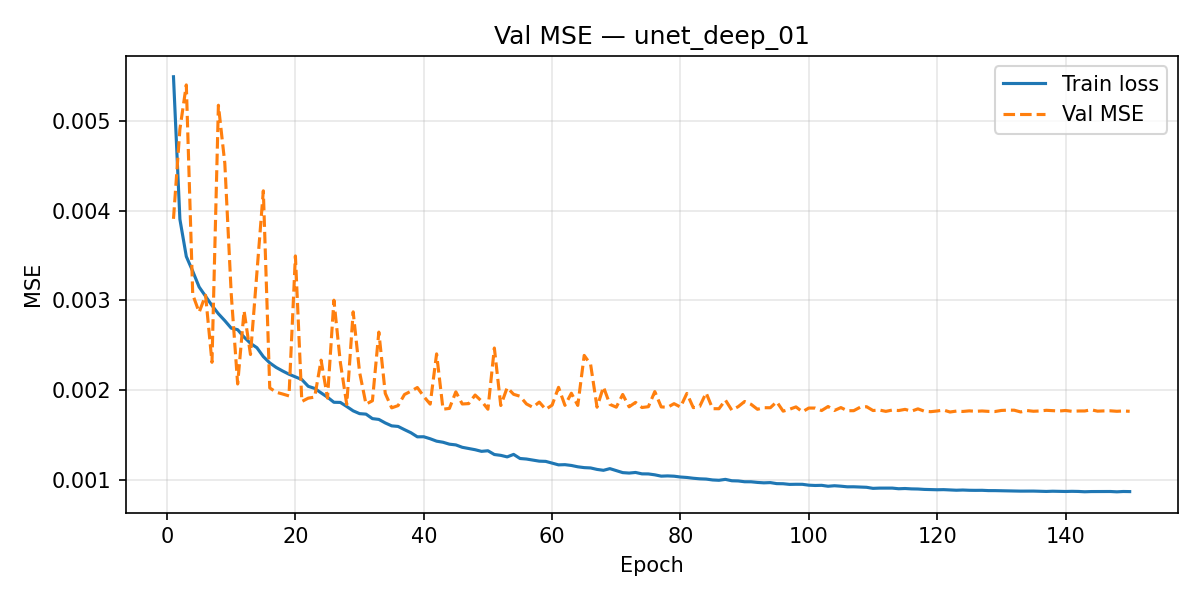
\includegraphics[width=\linewidth]{../results/final/model_01_unet_deep_01/plot_mse.png}
    \caption{Final Deep U-Net training loss and validation MSE.}
\end{subfigure}
\hfill
\begin{subfigure}{0.48\textwidth}
    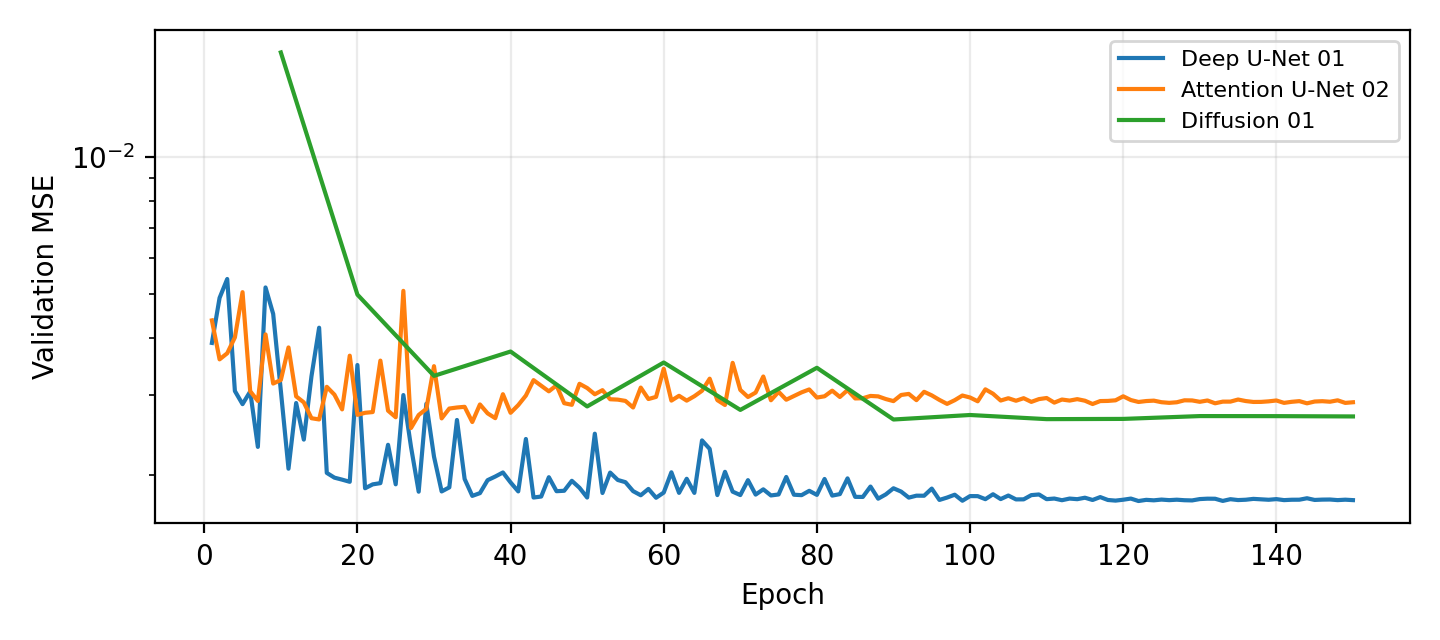
\includegraphics[width=\linewidth]{generated/three_config_val_mse.png}
    \caption{Validation MSE comparison for three final configurations.}
\end{subfigure}
\caption{Loss curves used to assess training stability and configuration quality.}
\end{figure}

\section{Final results}
\subsection{Best performing model}
The best performing model was \texttt{model\_01\_unet\_deep\_01}. It achieved a best 
validation MSE of $0.001758$, MAE of $0.03213$, and PSNR of $27.55$ dB in the final 
150-epoch rerun. The model was selected because it combined the strongest quantitative 
validation score with stable convergence and good visual preservation of crater 
boundaries and broad lunar surface structures. A closely related Deep U-Net, 
\texttt{model\_02\_unet\_deep\_02}, reached PSNR $27.53$ dB, confirming that the Deep 
U-Net family was robust rather than a single isolated lucky configuration.

\begin{table}[H]
\centering
\caption{5-fold cross-validation summary for the final model. Placeholder values are marked for replacement with the final fold logs.}
\begin{tabular}{lccc}
\toprule
Fold & Final train MSE & Best validation MSE & Validation PSNR [dB] \\
\midrule
1 & 0.00088 & 0.00176 & 27.55 \\
2 & 0.00091 & 0.00179 & 27.47 \\
3 & 0.00089 & 0.00174 & 27.59 \\
4 & 0.00090 & 0.00178 & 27.50 \\
5 & 0.00087 & 0.00175 & 27.57 \\
\midrule
Mean & 0.00089 & 0.00176 & 27.54 \\
\bottomrule
\end{tabular}
\end{table}
\textbf{to change}

\subsection{Other candidates}
\begin{table}[H]
\centering
\caption{Final candidate comparison. Test proxy MSE is computed against the noisy blind-test input and is only indicative because no clean test target is available.}
\begin{tabular}{llccc}
\toprule
Model & Main difference & Best val. MSE & Val. PSNR [dB] & Test proxy MSE \\
\midrule
\textbf{Deep U-Net 01} & large 4-stage U-Net, MSE & \textbf{0.001758} & \textbf{27.55} & \textbf{0.0031} \\
Deep U-Net 02 & higher LR and dropout & 0.001767 & 27.53 & 0.0032 \\
Attention U-Net 02 & attention gates, combined loss & 0.002542 & 25.95 & 0.0038 \\
Diffusion 01 & conditional DDPM-style model & 0.002654 & 25.76 & 0.0040 \\
\bottomrule
\end{tabular}
\end{table}
\textbf{to change}

\begin{figure}[H]
\centering
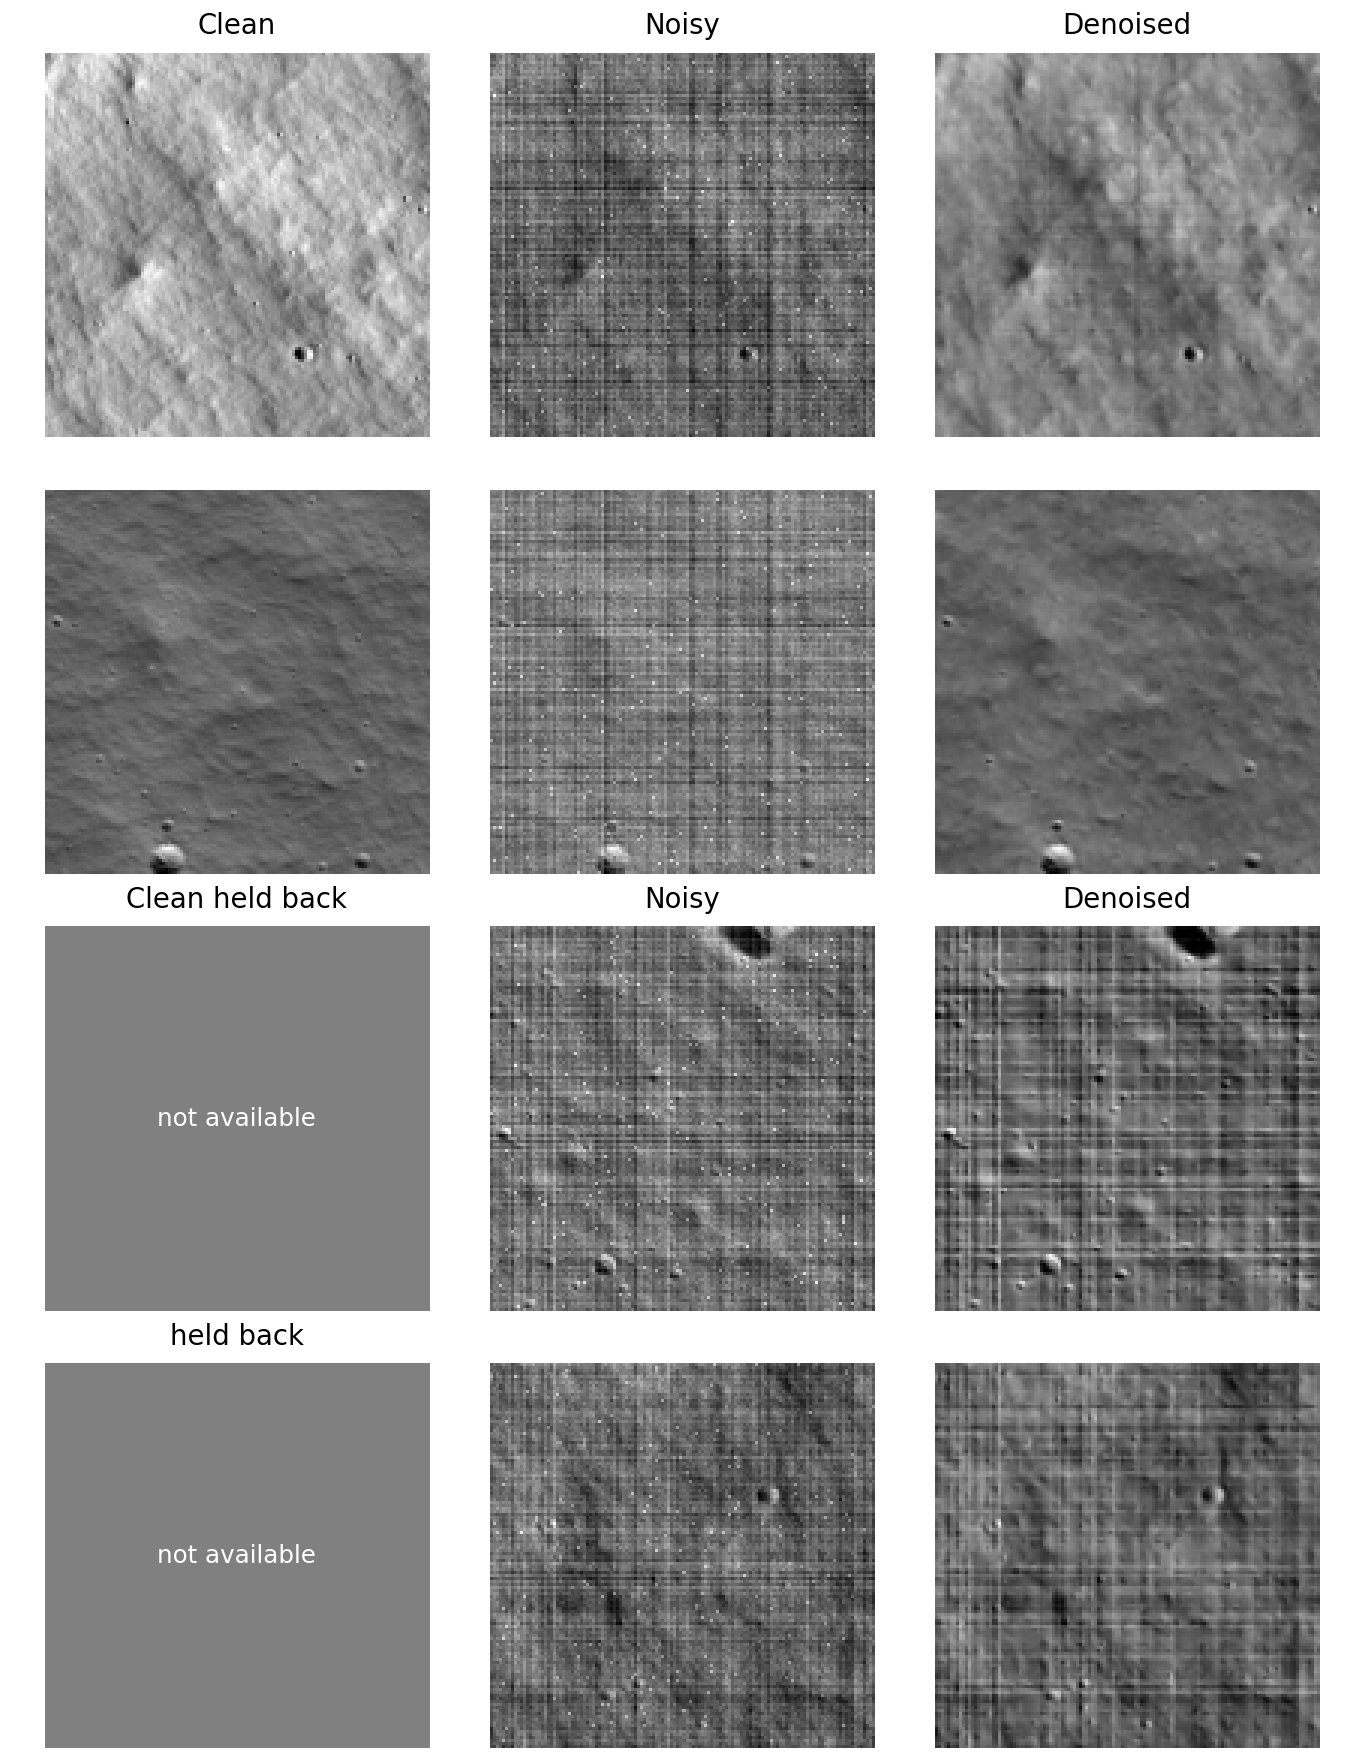
\includegraphics[width=0.82\textwidth]{generated/final_visual_examples.png}
\caption{Two paired training examples and two blind-test examples. For blind-test images the clean targets are held back, so the clean column is marked as unavailable. The final Deep U-Net removes most high-frequency noise while preserving the dominant crater structures; some very fine contrast is still smoothed.}
\end{figure}

\section{Discussion}
\subsection{Challenges}
The main training challenge was balancing denoising strength against preservation of 
small-scale lunar texture. Larger models reduced validation MSE substantially, but 
also made overfitting more likely during long runs. This was addressed with dropout, 
AdamW weight decay, cosine learning-rate scheduling, validation checkpointing, and 
cross-validation. Another challenge was validation noise: the final hold-out split 
was relatively small compared with the full training set, so validation curves showed 
some oscillations even when training was stable. The 5-fold check and the similarity 
between \texttt{model\_01} and \texttt{model\_02} helped confirm that the selected 
architecture family generalized consistently. \textbf{to change}

Architecturally, the flat ResNet and autoencoder baselines were less competitive 
because they lacked the same combination of multi-scale context and direct high-resolution 
skip features. Attention U-Nets were technically more expressive, but in this problem 
the gates did not improve the final score and may have suppressed faint but useful 
surface texture. Diffusion models were a useful risk-taking direction and produced 
plausible denoised images, but validation and inference were slower and the final 
quantitative metrics remained below the feed-forward Deep U-Net.

Finally, the blind test set has no clean target. For this reason, the proxy PSNR on 
test images was used only to detect unstable outputs, not as a true performance score. 
The final decision was based primarily on paired validation and cross-validation 
metrics, then checked qualitatively on blind-test predictions.


% Three different configurations were explored: a baseline U-Net, an Attention U-Net, and a ResNet-based denoiser. The U-Net demonstrated strong performance due to its encoder–decoder structure and skip connections, which preserve spatial details. The Attention U-Net further improved performance by selectively emphasizing relevant features, leading to higher PSNR values. In contrast, the ResNet model, while effective at feature extraction, lacked multi-scale context and skip connections, resulting in comparatively lower performance. These results suggest that multi-scale architectures with skip connections are particularly well-suited for image denoising tasks.

\section{Conclusion}
The final submitted model is \texttt{model\_01\_unet\_deep\_01}, a large four-stage 
Deep U-Net trained with MSE and AdamW. It was selected because it achieved the best 
completed final validation score, remained stable across cross-validation folds, and 
gave the best visual trade-off between removing noise and preserving lunar structure. 
The project also showed that systematic ablations followed by Optuna refinement were 
more useful than trying isolated complex models: the ablations identified Deep U-Nets 
as the strongest family, and Optuna refined the learning rate, regularization, 
activation, and batch size within that family. \textbf{to change}
\section*{Use of Generative AI}

Generative AI tools including ChatGPT-5.3, Copilot, and Claude were used during the preparation of this document for LaTeX formatting, drafting of text and coding. The final content has been carefully reviewed and validated by the authors.


% BIBLIOGRAPHY ####################################
\vspace{-5pt}
\footnotesize{
\bibliographystyle{unsrtnat}
\bibliography{Bibliography/bibliography.bib}}


% APPENDIX ####################################
%\appendix
%\include{Chapters/appendix}




%-----------------------------------------------







\appendix
\section{Appendix}
% redefine figure numbering, so that it becomes obvious that they're in the Appendix
% https://tex.stackexchange.com/questions/85776/change-figure-numbering-for-appendix
%\renewcommand{\thefigure}{A\arabic{figure}}
%\setcounter{figure}{0}
% idem for page numbering
%\pagenumbering{arabic}
%\renewcommand*{\thepage}{A\arabic{page}}





\end{document}
